\subsection{Construction of Confidence Intervals: A General Method}
\label{subsec:const-of-conf-inter-a-gen-method}

Given a sample of data and a desired confidence level $(1 - \alpha)$, how can we construct a confidence interval $\left[ a,\ b \right]$ that will satisfy the coverage condition
\begin{equation*}
  \prob{a \leq \theta \leq b} = 1 - \alpha
\end{equation*}
in definition 4.

We start by estimating parameter $\theta$. Assume there is an unbiased estimator $\hat{\theta}$ that has a Normal distribution. When we standardize it, we get a Standard Normal variable
\begin{equation*}
  Z = \frac{\hat{\theta} - \mathbf{E}(\hat{\theta})}{\sigma(\hat{\theta})} = \frac{\hat{\theta} - \theta}{\sigma(\hat{\theta})}
\end{equation*}
where $\mathbf{E}(\hat{\theta}) = \theta$ because $\hat{\theta}$ is unbiased, and $\sigma(\hat{\theta}) = \sigma(\hat{\theta})$ is its standard error.

\vspace*{\fill}
\columnbreak

This variable falls between the Standard Normal quantiles $q_{\alpha/2}$ and $q_{1 - \alpha/2}$, denoted by
\begin{align*}
  - z_{\alpha/2} &= q_{\alpha / 2}\\
  z_{\alpha/2} &= q_{1 - \alpha / 2}\\
\end{align*}
with probability $(1 - \alpha)$, see Figure 3.
\begin{figure}[H]
  \centering
  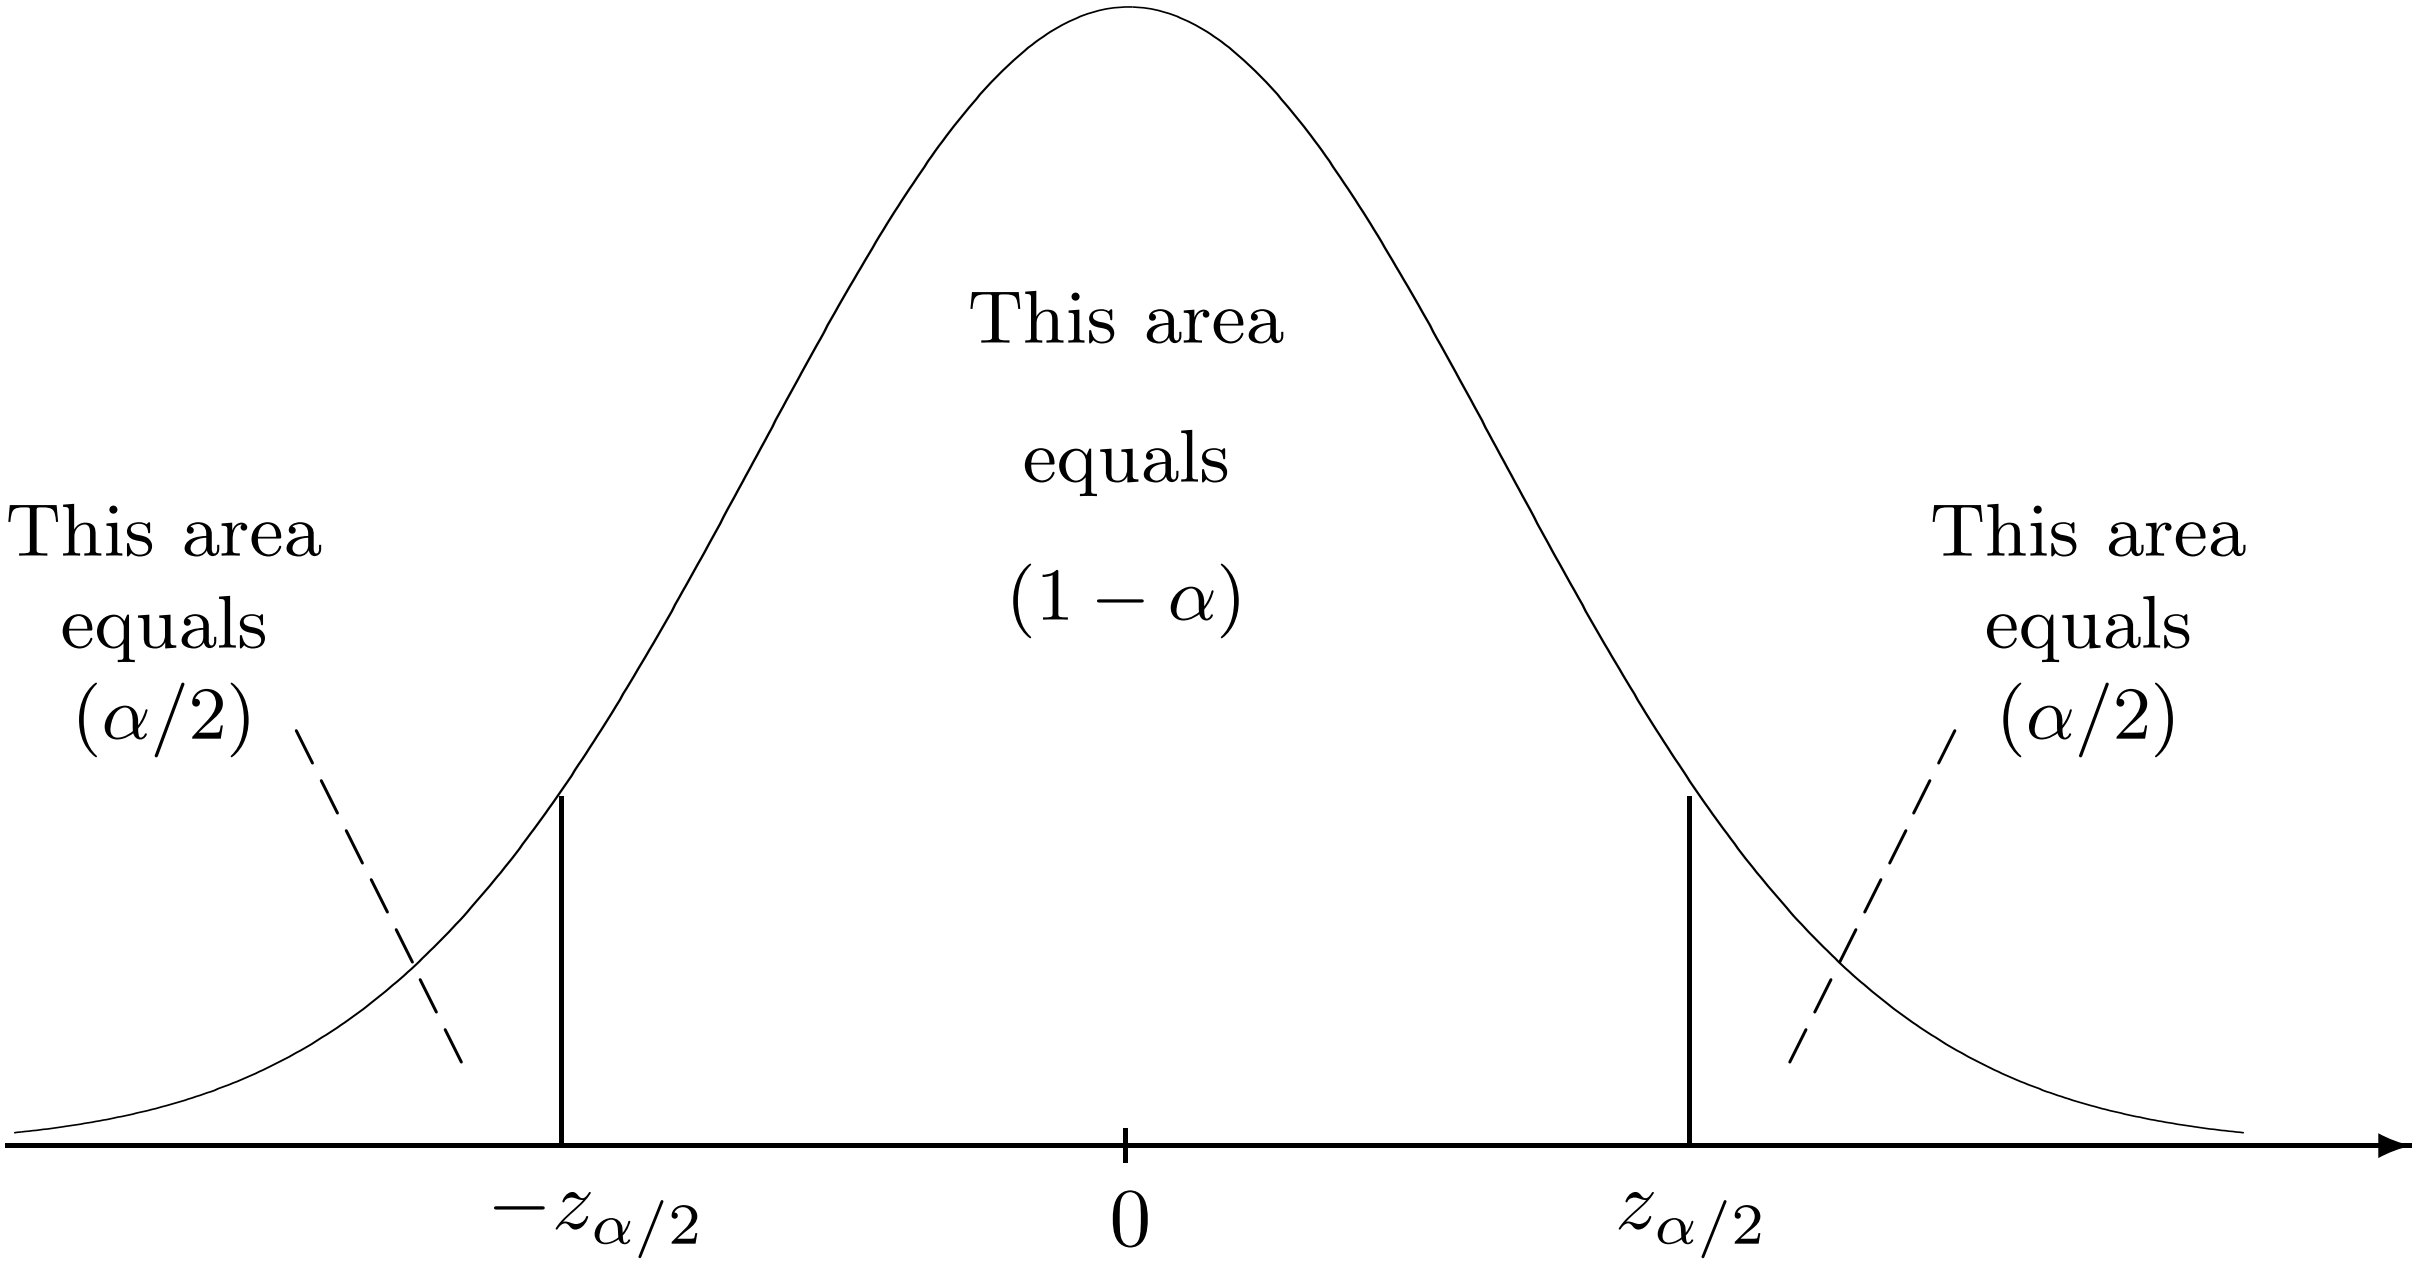
\includegraphics[width=\linewidth]{img/fig-9.3.png}
  \caption{}
  \label{fig:9.3}
\end{figure}

\noindent Then,
\begin{equation*}
  \prob{- z_{\alpha/2} \leq \frac{\hat{\theta} - \theta}{\sigma(\hat{\theta})} \leq z_{\alpha/2}} = 1 - \alpha
\end{equation*}
\noindent Solving the inequality inside $\{ \ldots \}$ for $\theta$, we get
\begin{equation*}
  \prob{
    \hat{\theta} - z_{\alpha/2} \cdot \sigma(\hat{\theta})
    \leq 
    \theta
    \leq
    \hat{\theta} + z_{\alpha/2} \cdot \sigma(\hat{\theta})
  } = 1 - \alpha
\end{equation*}
\noindent The problem is solved! We have obtained two numbers
\begin{align*}
  a &= \hat{\theta} - z_{\alpha/2} \cdot \sigma(\hat{\theta})\\
  b &= \hat{\theta} + z_{\alpha/2} \cdot \sigma(\hat{\theta})
\end{align*}
\noindent such that
\begin{equation*}
  \prob{a \leq \theta \leq b} = 1 - \alpha
\end{equation*}

\begin{formula}{Confidence interval, Normal distribution, Eq. 3}
  If parameter $\theta$ has an unbiased, Normally distributed estimator $\hat{\theta}$, then
  \begin{equation*}
    \hat{\theta} \pm z_{\alpha/2} \cdot \sigma(\hat{\theta}) = \left[ \hat{\theta} - z_{\alpha/2} \cdot \sigma(\hat{\theta}), \hat{\theta} + z_{\alpha/2} \cdot \sigma(\hat{\theta}) \right]
  \end{equation*}
  is a $(1 - \alpha)100\%$ confidence interval for $\theta$.

  If the distribution of $\hat{\theta}$ is \textit{approximately} Normal, we get an approximately $(1 - \alpha)100\%$ confidence interval.
\end{formula}

\setcounter{equation}{4}

In this formula, $\hat{\theta}$ is the \textbf{center of the interval}, and $z_{\alpha/2} \cdot \sigma(\hat{\theta})$ is the \textbf{margin}. The margin of error is often reported along with poll and survey results. In newspapers and press releases, it is usually computed for a $95\%$ confidence interval.

\begin{formula}{NOTATION}
  \begin{equation*}
    z_{\alpha} = q_{1 - \alpha} = \Phi^{-1} (1 - \alpha)
  \end{equation*}
  is the value of a Standard Normal variable $Z$ that is exceeded with probability $\alpha$
\end{formula}

\noindent Several important applications of this general method are discussed below. In each problem, we
\begin{enumerate}
  \item Find an unbiased estimator of $\theta$,
  \item Check if it has a Normal distribution,
  \item Find its standard error $\sigma(\hat{\theta}) = \textnormal{Std}(\hat{\theta})$,
  \item Obtain quantiles $\pm z_{\alpha/2}$ from the table of Normal distribution (Table A4 in the Appendix in textbook), and finally,
  \item Apply the rule (3).
\end{enumerate}